\subsection{Adeline}

\begin{frame}
\frametitle{\underline{ADA}ptive \underline{LIN}ear \underline{E}lement}

\comment{
\begin{itemize}
\item \textbf{ADA}ptive \textbf{LIN}ear \textbf{E}lement
\item Verzicht auf die Einheits-Sprungfunktion 
\item Stattdessen Nutzung linearer Aktivierungsfunktion 
\begin{itemize}
	\item wird erst einmal mit der Identiätsfunktion bestzt
\end{itemize}
\item Klassifizierungs- bzw. Entscheidungsfunktion im letzten Schritt
\begin{itemize}
	\item irrelevant für Trainingsalgorithmus
\end{itemize}
\end{itemize}
}

\begin{figure}
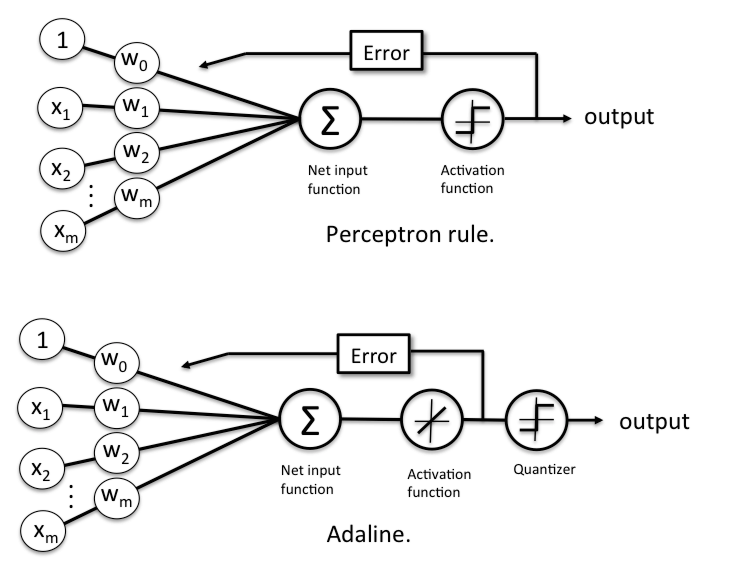
\includegraphics[width=.9\linewidth]{./geschichtliches/adeline/img/adeline_aufbau}
\end{figure}

\end{frame}


\begin{frame}
\frametitle{Delta-Regel}

\begin{itemize}
\item Leralgorithmus durch Erfinder geprägt
\item auch unter \emph{Least-Mean-Square}-Algrithmus bekannt
\item Wesentlicher Vorteil: Ableitbare Kostenfunktion
\end{itemize}

\hspace{2mm}

\begin{block}{Notation}
\begin{align*}
J(w)  = \frac{1}{2} \sum_{i} (\text{target}^{(i)} - \text{output}^{(i)})^2 \quad \quad \text{output}^{(i)} \in \mathbb{R} \\
\end{align*}
\end{block}

\end{frame}



\begin{frame}
\frametitle{Gradientenverfahren}

\hspace{1.5mm}

\begin{itemize}
\item Ziel: Gradientenvektor für bestimmten Input bestimmen: $\nabla J \equiv \left(\frac{\partial J}{\partial w_1}, \ldots, \frac{\partial J}{\partial w_m}\right)^T.$
\end{itemize}


\begin{figure}
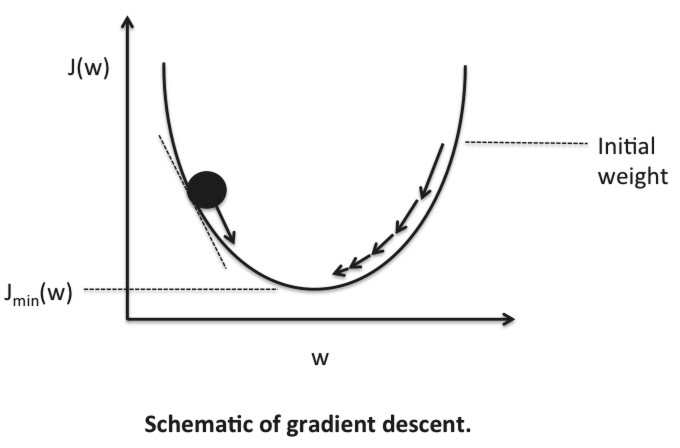
\includegraphics[width=.8\linewidth]{./geschichtliches/adeline/img/adeline_gd1_alpha}
\end{figure}

\end{frame}


\begin{frame}
\frametitle{Partielle Ableitungen}

\begin{columns}

\column{0.5\textwidth}
\begin{itemize}
\item Differenzieren von Funktionen mit mehreren Eingabewerten
\item Beispiel: $z = f(x) = x^2 + y^2$
\end{itemize}

\hspace{2mm}

\begin{block}{Partielle Ableitung - Notation}
\begin{align*}
\frac{\partial Abzuleitende Fkt.}{\partial Betrachtete Komponente}
\end{align*}
\end{block}

\column{0.5\textwidth}
\begin{figure}
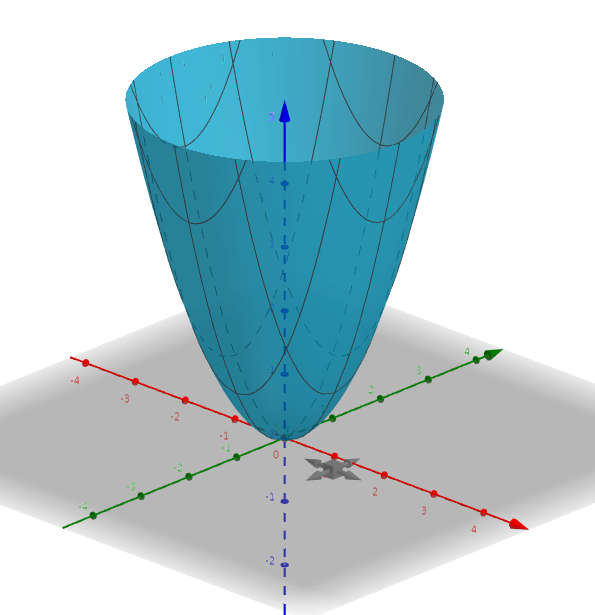
\includegraphics[width=\linewidth]{./geschichtliches/adeline/img/partAbl_1_alpha}
\end{figure}

\end{columns}
\end{frame}



\begin{frame}
%\frametitle{Partielle Ableitungen}

\begin{columns}
\column{0.65\textwidth}
\begin{figure}
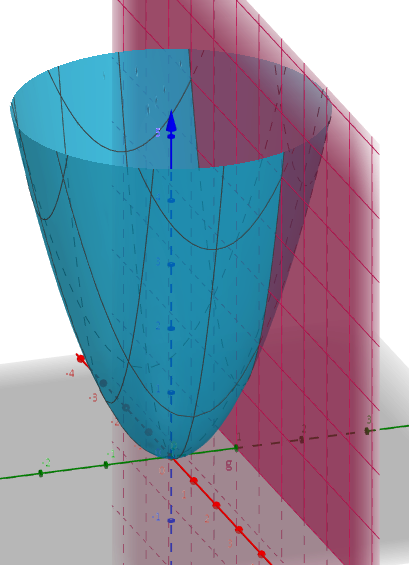
\includegraphics[width=.78\linewidth]{./geschichtliches/adeline/img/partAbl_2_alpha}
\end{figure}

\column{0.45\textwidth}
\begin{figure}
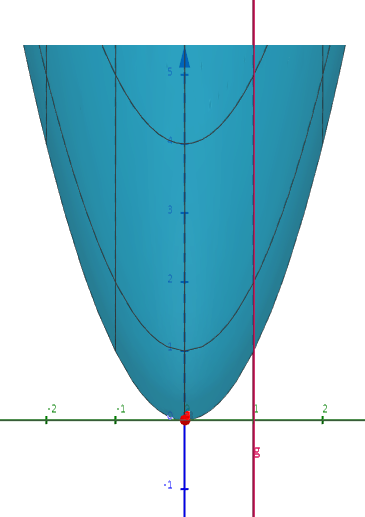
\includegraphics[width=.6\linewidth]{./geschichtliches/adeline/img/partAbl_3_alpha}
\end{figure}

\begin{block}{Ableitung - Beispiel}
\begin{align*}
\begin{aligned}
& z = f(x, y) = x^2 + y^2 \\
& \frac{\partial z}{\partial x} = 2x \;\;\;\;\; \frac{\partial z}{\partial y} = 2y 
\end{aligned}
\end{align*}
\end{block}

\end{columns}



\end{frame}


\begin{frame}
\frametitle{Gradientenverfahren}

\begin{figure}
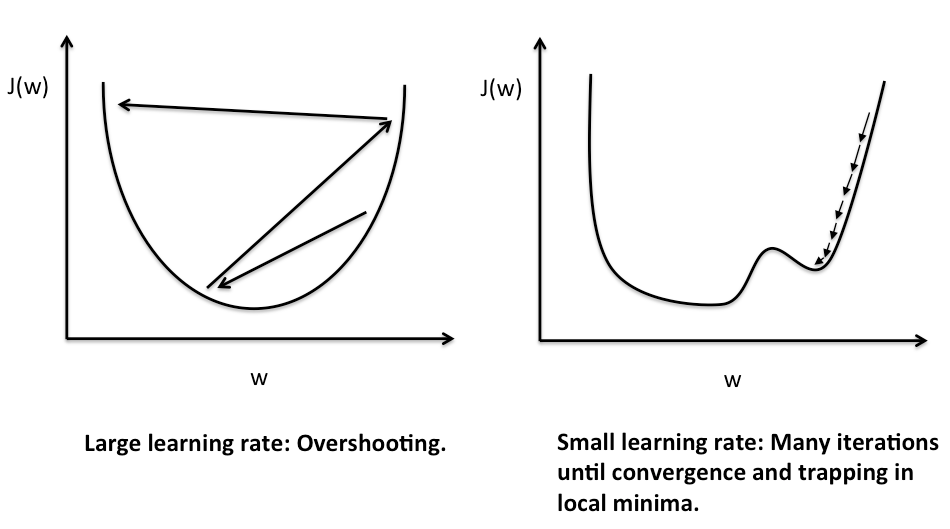
\includegraphics[width=\linewidth]{./geschichtliches/adeline/img/adeline_learning_rate_alpha}
\end{figure}

\end{frame}


\begin{frame}
\frametitle{Gradientenverfahren}
\begin{figure}
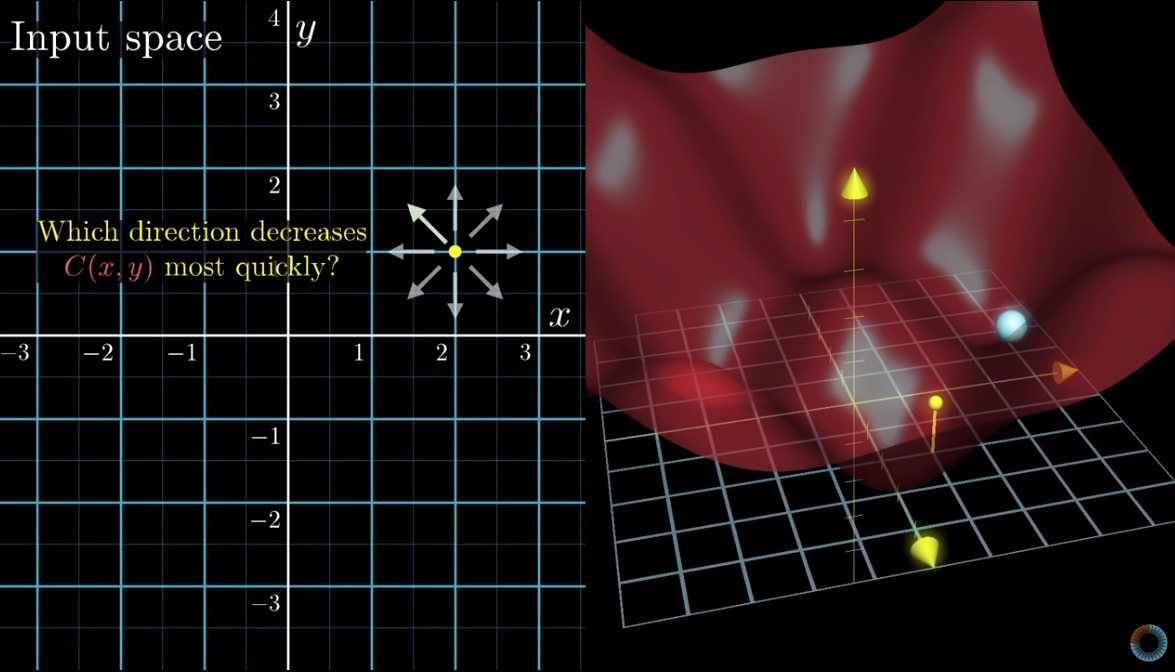
\includegraphics[width=\linewidth]{./geschichtliches/adeline/img/3dPlot_1}
\end{figure}
\end{frame}


\begin{frame}
\frametitle{Gradientenverfahren}
\begin{figure}
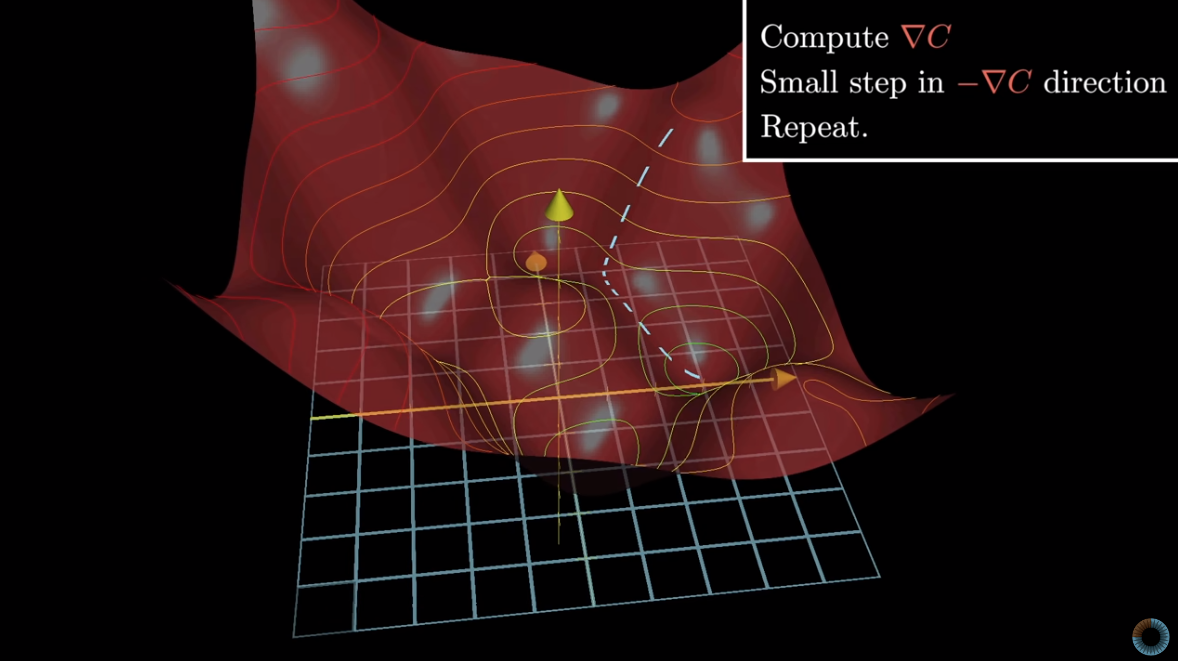
\includegraphics[width=\linewidth]{./geschichtliches/adeline/img/3dPlot_2}
\end{figure}
\end{frame}


\begin{frame}
\frametitle{Gradientenverfahren}

\begin{block}{Gradientenverfahren - Anwendung}

\begin{itemize}

\item Gradientenvektor
\begin{align*}
\nabla J \equiv \left(\frac{\partial J}{\partial w_1}, \ldots, \frac{\partial J}{\partial w_m}\right)^T.
\end{align*}

\item Allgemein: Vektorielle Darstellung
\begin{align*}
\Delta w = - \eta \nabla J(w)
\end{align*}

\comment{$
\!
\begin{aligned}[t]
\Delta w = - \eta \nabla J(w)
\end{aligned}
$}

\item Für die jeweiligen Gewichte: Komponentenweise Darstellung
\begin{align*}
\Delta w_j = - \eta \frac{\partial J}{\partial w_j}
\end{align*}
\end{itemize}
\end{block}


\begin{itemize}
\item Angleichung der Gewichte $w = w + \Delta w$
\end{itemize}

\end{frame}



\begin{frame}
\frametitle{Kostenfunktion ableiten}

\begin{align*}
\frac{\partial J}{\partial w_j} & = \frac{\partial }{\partial w_j} \frac{1}{2} \sum_i  (t^{(i)} - o^{(i)})^2 \\
 & = \frac{1}{2} \sum_i \frac{\partial }{\partial w_j} (t^{(i)} - o^{(i)})^2 \\
 & = \frac{1}{2} \sum_i 2 (t^{(i)} - o^{(i)}) \frac{\partial }{\partial w_j} (t^{(i)} - o^{(i)}) \\
 & = \sum_i (t^{(i)} - o^{(i)}) \frac{\partial }{\partial w_j} \bigg(t^{(i)} - \sum_j w_j x^{(i)}_{j}\bigg) \\
 & = \sum_i  (t^{(i)} - o^{(i)})(-x^{(i)}_{j})
\end{align*}




\end{frame}

